%\section{Memory management}
This section discusses how memory is managed in the microcontroller. Programs for many embedded systems - especially ones with only a small amounts of memory available - only allocates memory to variables statically, before the program is executed. In the application written for the microcontroller in this project, most programmer-defined variables are static. Not all are, however, and the FreeRTOS kernel itself also uses dynamic memory allocation when creating new tasks, queues and the like. 


\subsection{Memory map}
The LM3S6965 microcontroller has 65 kB on-chip SRAM. That memory lies from address \texttt{0x20000000} to \texttt{0x20010000} \cite[71]{lm3s6965} and is where the data and BSS segments are contained. Additionally, the SRAM holds the stack and heap. Figure \ref{fig:memmap} displays a graphical representation of how the SRAM looks for a debug build. The data segment holds global and static variables that are explicitly initialized with a value. The BSS segment contains global or static variables which are uninitialized. The start-up code maps the data segment values from flash into SRAM and initializes the BSS area to zero.

\begin{figure}[htb]
	\centering
	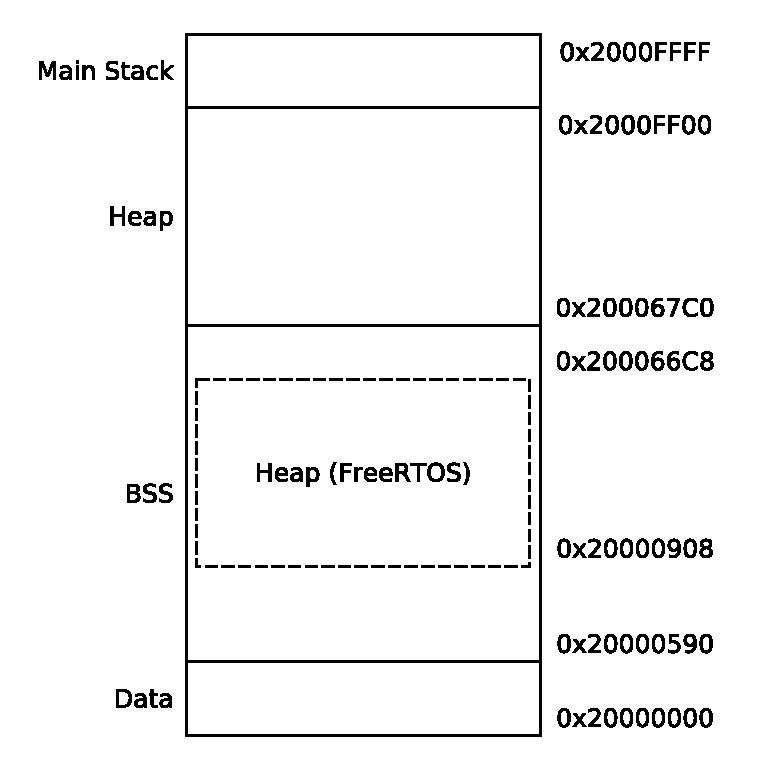
\includegraphics[scale=0.66,trim=0 0 0 0]{memorymap.pdf}%trim=l b r t
	\caption{Map of the SRAM for a debug build (commit \texttt{5e3d6c3e} on the Git tree).}
	\label{fig:memmap}
\end{figure}

Studying figure \ref{fig:memmap} one will notice that the heap used by FreeRTOS also resides in the BSS segment. This is because the FreeRTOS \texttt{heap\_2.c} memory allocation scheme declares the heap it uses as a large static array.

In the current implementation of the microcontroller application, both of the two heaps are used. At first only the FreeRTOS heap was defined, but along the way the need to use FreeRTOS' \texttt{vTaskGetRunTimeStats} function call arose. The function to print runtime statistics uses whatever \texttt{sprintf} function is available to generate formatted strings. On our system, using the GNU C Compiler to cross compile for the ARM Cortex-M3, \texttt{sprintf} is supplied by the Newlib C library implementation. The Newlib \texttt{sprintf} in turn uses Newlibs own \texttt{malloc} to dynamically allocate memory. This is where the second heap area comes in.

The second heap is quite simply two symbols defined in the linker script, marking the beginning and end of that memory area.


\subsection{Memory allocation schemes}
At the moment of writing, the microcontroller application uses both \texttt{pvPortMalloc} as implemented in \texttt{heap\_2.c} and \texttt{malloc} as it is implemented in Newlib. Here we'll take a short look at the two memory allocators and some of the differences between them.

The simplest of the two allocation schemes is FreeRTOS' \texttt{pvPortMalloc} (\texttt{heap\_2.c}). It works by dividing the static array, which it uses as heap, into smaller blocks. Initially the array is just one large block. When a call is made to \texttt{pvPortMalloc}, the large block is split. The size of the smaller blocks depends on how much memory is requested. Each memory block has a header which contains the size of that particular block and a pointer to the header of the next free block. The headers of the memory blocks form a linked list. When a memory allocation request is made, that linked list is traversed until a block of adequate size is found. Since the items in the linked list are sorted by the size of the memory block, the allocation algorithm is essentially a ``best fit'' algorithm. A call to \texttt{vPortFree} frees the memory block in question, but does not re-combine adjacent blocks. Nothing is done to prevent fragmentation, which allows a very fast way of freeing memory, but would cause problems if the application were to allocate and free blocks of unpredictable size.

The Newlib \texttt{malloc} implementation is more advanced. It is based on ``Doug Lea's Malloc'' \cite{dlmalloc}, which is widely used. The allocator will not be described in great detail here, as it would be beyond the scope of this report. However, some of it's main advantages and disadvantages, compared to the FreeRTOS \texttt{pvPortMalloc}, will be discussed.

The Newlib allocator allocates memory on the heap as \textit{chunks}, which is somewhat similar to what the FreeRTOS allocator does. There are some significant differences though: Unallocated chunks are grouped in \textit{bins} of fixed sizes. There are 128 bins in total. One of the main differences between the FreeRTOS and Newlib allocators is, that the Newlib allocator coalesces adjacent blocks, or chunks, of memory into one. They are then held in the bins, which are searched in size order. Special care is taken to improve efficiency, especially with regard to coalescing adjacent chunks of memory, by, for example, storing the size of the chunk both in the beginning and end of it.

As such, the FreeRTOS allocator is likely to be the fastest, but not necessarily the most efficient. It very much depends on the way the application works. If only memory blocks of fixed sizes are dynamically allocated, and the memory is not fragmented too much, the FreeRTOS allocator is probably the best, requiring the least overhead and being the fastest. On the other hand, if the size and order of memory requests are unpredictable, the Newlib allocator will most likely be better. Especially after the microcontroller has run for a long time, fragmentation could become a big problem and might render large parts of the memory unusable or at least increase search time to find free blocks.


\subsection{Use in this application}
In this application, the only time the Newlib allocator is used, is when generating runtime statistics through a call to \texttt{vTaskGetRunTimeStats}. This is in fact also the only place where allocations of unknown size could take place. All other allocations are memory for tasks, queues, SPI user buffers and UI menu items. These are of a known size, which can be determined with the \texttt{sizeof} operator at compile-time. The number and order of allocations is pre-determined.

There is a downside to using two heap areas and two allocator implementations though. If a memory area larger than the available space in \textit{one} of the heaps were to be requested, there would be no way of allocating it. Had there been one large heap instead, the request could have been successful. Using two allocator implementations also increases code size, which could be problem if the program had been so large, that there was no longer enough flash memory in the microcontroller.

\nomenclature{SRAM}{Static Random-Access Memory}
